\section{Koblingsagentens påvirkning på ``Good Stuff''}
\label{sec:koblingsagent}
Som nevnt tidligere vil en automatisk koblingsagent ha stor påvirkning på firmaet som driver ``Gi bort dagen". Først og fremst vil koblingsagenten påvirke i form av redusert ressursbehov på grunn av færre arbeidstimer for å manuelt koble givere med mottakere. I tillegg til lavere ressursbruk, vil en koblingsagent bidra til at ``Gi bort dagen" blir et mer fullstendig produkt som er lettere å presentere og markedsføre både til potensielle mottakere og givere, men også til eventuelle økonomiske bidragsytere.

``Good Stuff" vil, som alle andre bedrifter, avhenge av å være bærekraftig. Dette betyr at de må ha inntekter som tilsvarer eller overstiger kostnadene. I det norske næringslivet er lønnskostnader en av de aller største kostnadsdriverne. Det å kunne minimere disse vil derfor i stor grad bidra til bærekraftighet. En automatisk koblingsagent vil forenkle mye av matchingen mellom mottakere og givere. Det vil ikke være nødvendig med flere ansatte selv om prosjektet vokser da koblingsagenten foreslår gode matcher og mottaker og giver selv kontakter hverandre uten involvering av ``Good Stuffs" ansatte. Dette faktum vil være en stor forbedring fra dagens situasjon hvor ``Engasjert Byrås" ansatte har brukt mye tid på å manuelt finne gode matcher. Arbeidet var overkommelig det første året, men ettersom konseptet ble mer populært har matchingsarbeidet nærmest blitt uoverkommelig, spesielt tatt i betraktning at ``Gi bort dagen" ikke har gitt ``Engasjert Byrå"" økte inntekter. Det vil naturligvis være nødvendig med ansatte for å drifte og vedlikeholde koblingsagenten. Likevel vil behovet for ansatte være uavhengig av omfanget til prosjektet, noe som bidrar til et mye mer skalerbart produkt.

Utover muligheten til å påvirke kostnadene til ``Good Stuff", har koblingsagenten også mulighet til å påvirke potensiell inntekt. Gjennom implementering av en automatisk koblingsagent vil “Gi bort dagen”-konseptet bli mye mer komplett. Markedsføringen av konseptet vil forenkles fordi man har noe mer håndfast og strukturert å henvise til. ``Gi bort dagen" vil i mye større grad kunne fremstilles som et fullstendig produkt i og med at koblingene er standardiserte og mye mindre påvirket av ``Good Stuffs" ansatte. Håpet er at dette vil forenkle prosessen med å selge konseptet til potensielle økonomiske bidragsytere, men også å øke mulighetene for annonsering. Annonsering vil være aktuelt i to former, annonsering og linker til koblingsagenten på eksterne sider som VG.no og adressa.no, men også annonser for andre firmaer på ``Gi bort dagens" hjemmeside. Skalerbarhet og standardisering er noen av de viktigste nye egenskapene ved konseptet som følge av en automatisk koblingsagent. Dette er egenskaper som er viktige for eventuelle økonomiske bidragsytere i forbindelse med en beslutning om investering, og dermed bedrer sjansene for flere investorer.

Utover muligheten for økte sjanser for økonomiske bidragsytere, vil koblingsagenten kunne bidra til nye forretningsmuligheter for ``Good Stuff". For eksempel vil alle mottakere og givere bli bedt om å fylle inn bedriftens/organisasjonens verdier i forbindelse med koblingsprosessen. Dette kan være svært verdifullt for “Good Stuff” da de kan foreslå og tjene penger på rådgiving til firmaer som mangler slike organisasjonsverdier.

En annen inntekstmulighet som koblingsagenten gir er at man som giver må betale en fast avgift for å registrere seg. Denne faste avgiften bør variere avhengig av bedriftens størrelse og omsetning slik at den ikke blir et hinder for å delta, men snarere en symbolsk sum. Et slikt opplegg vil betydelig forbedre “Good Stuffs” bærekraftighet så lenge summen ikke er så høy at den reduserer villigheten til å bidra.

Det er nå pekt på koblingsagentens effekter for ``Good Stuff". Figur \ref{fig:koblingsagentMuligheter} illustrerer mulighetene som følger av implementering av en koblingsagent og det overordnede resultatet av disse; bærekraftighet.

\begin{center}
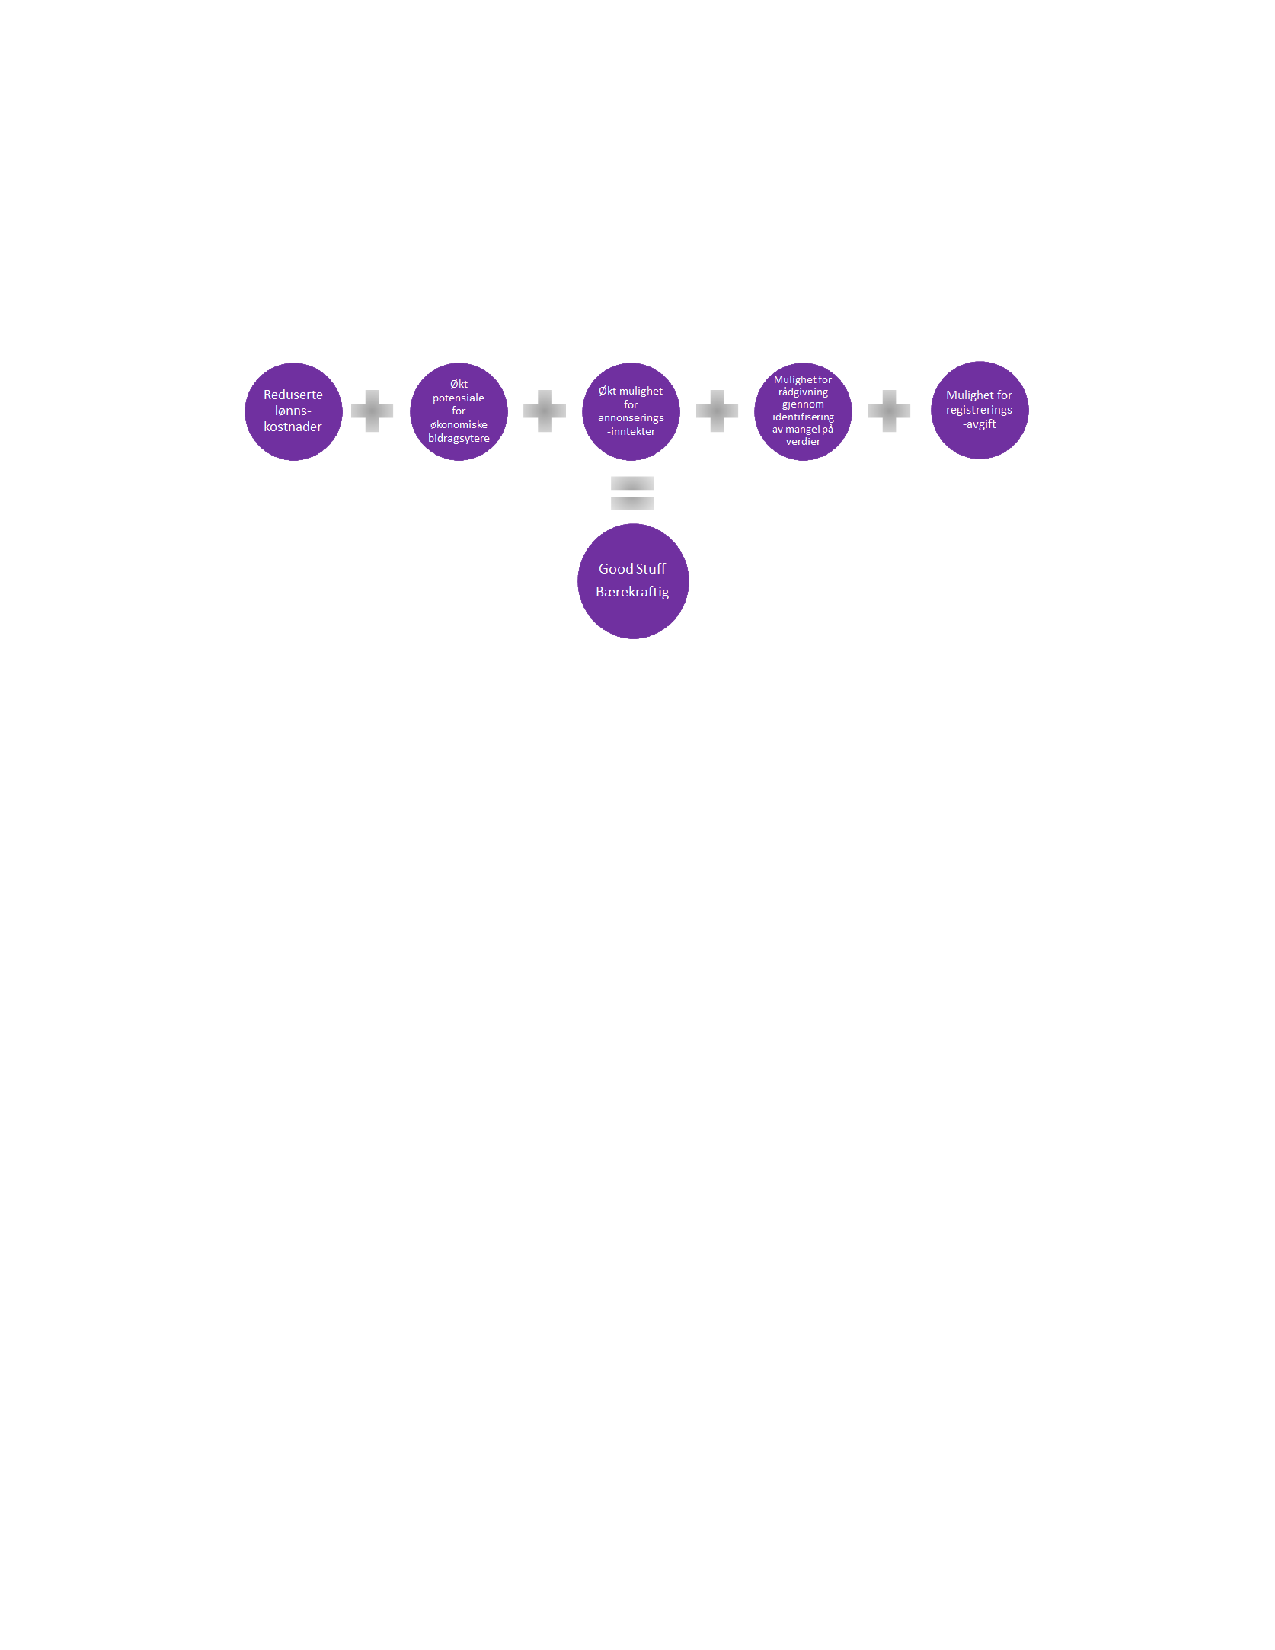
\includegraphics[clip=true, width=1 \textwidth,
trim=4cm 16cm 4cm 4cm]{koblingsagentMuligheter.pdf}
\captionof{figure}{Muligheter og resultat av en automatisk koblingsagent}
\label{fig:koblingsagentMuligheter}
\end{center}

Vi kan dermed konkludere med at en automatisk koblingsagent vil ha en positiv effekt på ``Good Stuff" på flere måter som illustrert i figur \ref{fig:koblingsagentMuligheter}. Uten en automatisering av matchingsarbeidet mellom mottakere og givere i forbindelse med ``Gi bort dagen" vil det være vanskelig for ``Good Stuff" å videreutvikle prosjektet. På mange måter vil en automatisk koblingsagent derfor være kritisk for ``Gi bort dagens", og dermed også ``Good Stuffs" videre suksess.

\section{Andre bruksområder for koblingsagenten }
\label{sec:andrebruksomrader}
Hovedformålet med koblingsagenten er nøye fremstilt i andre deler av prosjektrapporten, men det er også viktig å se på hvilke andre potensielle områder et slikt produkt kan benyttes innenfor. Ved å få frem ulike potensielle bruksområder kan man se koblingsagenten i et større perspektiv, og i den anledning se muligheter for bærekraftighet og ``Good Stuff" som helhet. Under vil ulike bruksområder og produkter som vi har diskutert bli presentert.

\subsection{“Strekk ut hånden”}
\label{sec:strekkuthanden}
``Gi bort dagen" har selvfølgelig vært hovedfokuset gjennom vårt arbeid. Dette konseptet omhandler hovedsakelig organisasjoner og bedrifter som blir koblet sammen som mottakere og givere. Disse koblingene er gjerne av en viss størrelse, og omhandler ofte mange involverte personer. En mulig utvidelse av ``Gi bort dagen" kan derfor være det vi har valgt å kalle ``Strekk ut hånden".

``Strekk ut hånden" er et konsept som baserer seg på det samme prinsippet som ``Gi bort dagen" der frivillighet er i fokus. Den store forskjellen mellom disse to konseptene er størrelsen på mottakerne og giverne. I ``Strekk ut hånden" skal fokuset ligge mer på enkeltpersoner, og i hovedsak mindre oppgaver. Disse oppgavene kan være alt fra å hjelpe med flytting til leksehjelp.

Et viktig aspekt ved et slikt prosjekt er kompleksitet og størrelse. I ``Gi bort dagen" er områdene av frivillighet relativt begrenset, noe som gjør koblingsagenten til dels enkel å utarbeide. I en løsning rettet mot privatpersoner kan spennet av forespørsler være enormt. Dette setter krav til å utarbeide en smart løsning i koblingsagenten. En mulighet kan eventuelt være å begrense valgene brukerne får. Når man snakker om privatpersoner blir ofte personvern et viktig tema. Dette vil også være noe som må nøye vurderes hvis et slikt konsept skal realiseres.

I dag finnes det noen løsninger som fokuserer delvis på et slikt konsept. En lignende løsning som ble publisert for kort tid siden er FINN sine ``Småjobber". Her kan privatpersoner legge ut ønsket arbeid med en fastsatt betaling. Konseptet i seg selv er veldig likt det vi har tenkt på i forhold til ``Strekk ut hånden", dog vil en lignende inntektsmodell ikke være mulig mtp. ønsket om frivillighet. Mulige løsninger kan være private donasjoner eller sponsorer, eventuelt reklame.

En annen organisasjon som kan være verdt å nevne er ``Frivillig Trondheim". Denne organisasjonen arbeider for frivillighet opp mot ulike arrangementer som kan variere fra for eksempel idrettsarrangementer til konserter og festivaler. Det er viktig å poengtere at du her melder deg opp som en privatperson, men vil gjerne arbeide frivillig for en organisasjon. Et annet poeng er at lokaliseringen kun er i Trondheimsområdet.

\subsection{Barn og aktivitet}
\label{sec:barnaktivitet}
Et problem man ofte hører om i dagens samfunn er barn som føler seg utenfor, og barn som kjeder seg. Mange føler det er vanskelig å ta initiativet for å bli med i ulike aktiviteter som eksempelvis idretter. Vi fant derfor ut at en mulig idé kunne være å knytte barn og aktiviteter gjennom en koblingsagent.

Koblingene ville fungert veldig likt som koblingene i ``Gi bort dagen"-konseptet hvor organisasjonene som holder aktivitetene ville blitt givere, og barna som benyttet produktet ville vært plassert i kategorien mottakere. Med en slik løsning ville man kunne laget en lavterskel måte for barn å kunne bli innlemmet i aktiviteter. Samtidig vil det være en enkel måte for barna å prøve ut aktiviteter de kanskje har vært usikre på.

Et viktig aspekt i forhold til dette konseptet er sikkerhet. Det vil være veldig viktig å ha en god bakgrunnssjekk på alle organisasjoner som registrerer seg som givere. For at konseptet skal fungere må både barn og foreldre ha tillit til at systemet sikrer personopplysninger. Dette vil medføre at funksjonalitet må legges til i den nåværende koblingsagenten, og mest sannsynlig en manuell godkjenning av alle givere.

For at et slikt produkt skal være bærekraftig må man tenke nøye gjennom fremgangsmåten. En naturlig tankegang vil være å la organisasjonene som registerer seg som givere betale en liten avgift. Dog kan dette være problematisk for mindre organisasjoner. En annen løsning kan være statlig støtte som virker naturlig for et slikt konsept. Andre muligheter vil være donasjoner og reklame.

\subsection{iFriend}
\label{sec:iFriend}
Et tredje konsept som ble diskutert var iFriend. Et dagsaktuelt tema er personer som føler seg ensomme, og som kanskje har falt utenfor samfunnet. Idéen bak iFriend vil da være å kunne skape koblinger mellom personer som kunne trengt selskap for å minske ensomheten, og kanskje skape permanente relasjoner gjennom vennskap.

Konseptet vil basere seg på mange av de samme prinsippene som bak datingsider der matchingen vil foregå på parametere som hver enkelt person legger inn. Dette vil være naturlig for å kunne samle personer med noen fellestrekk, som eksempelvis interesseområder. En annen idé i det samme konseptet kan være å koble sammen flere personer i grupper. For mange kan det være vanskelig å åpne seg når man er på tomannshånd, og trenger flere rundt seg for å føle seg trygg. Det vil også ofte være enklere å gjøre aktiviteter sammen hvis man er en gruppe, og dersom enkelte medlemmer av gruppen ikke er tilgjengelig vil andre med stor sannsynlighet være det.

Som nevnt over vil konseptet ha mange fellestrekk med hvordan datingsider fungerer. Måten datingsider holder seg bærekraftig er oftest gjennom at brukerne betaler et visst beløp for å legge inn en annonse. I tillegg bruker ofte sidene reklamer som inntekt. Det vil kanskje være unaturlig at brukerne av iFriend skal betale for bruk av en slik tjeneste, men reklamer kan være et alternativ. En annen form for inntekt kan komme gjennom private sponsorer og donasjoner, eller statlig støtte hvis dette skulle være interessant for høyere hold.

Figur \ref{fig:automatiskKoblingsagent} nedenfor illustrerer de tre potensielle prosjektene hvor en automatisk koblingsagent kan benyttes utover “Gi bort dagen”.

\begin{center}
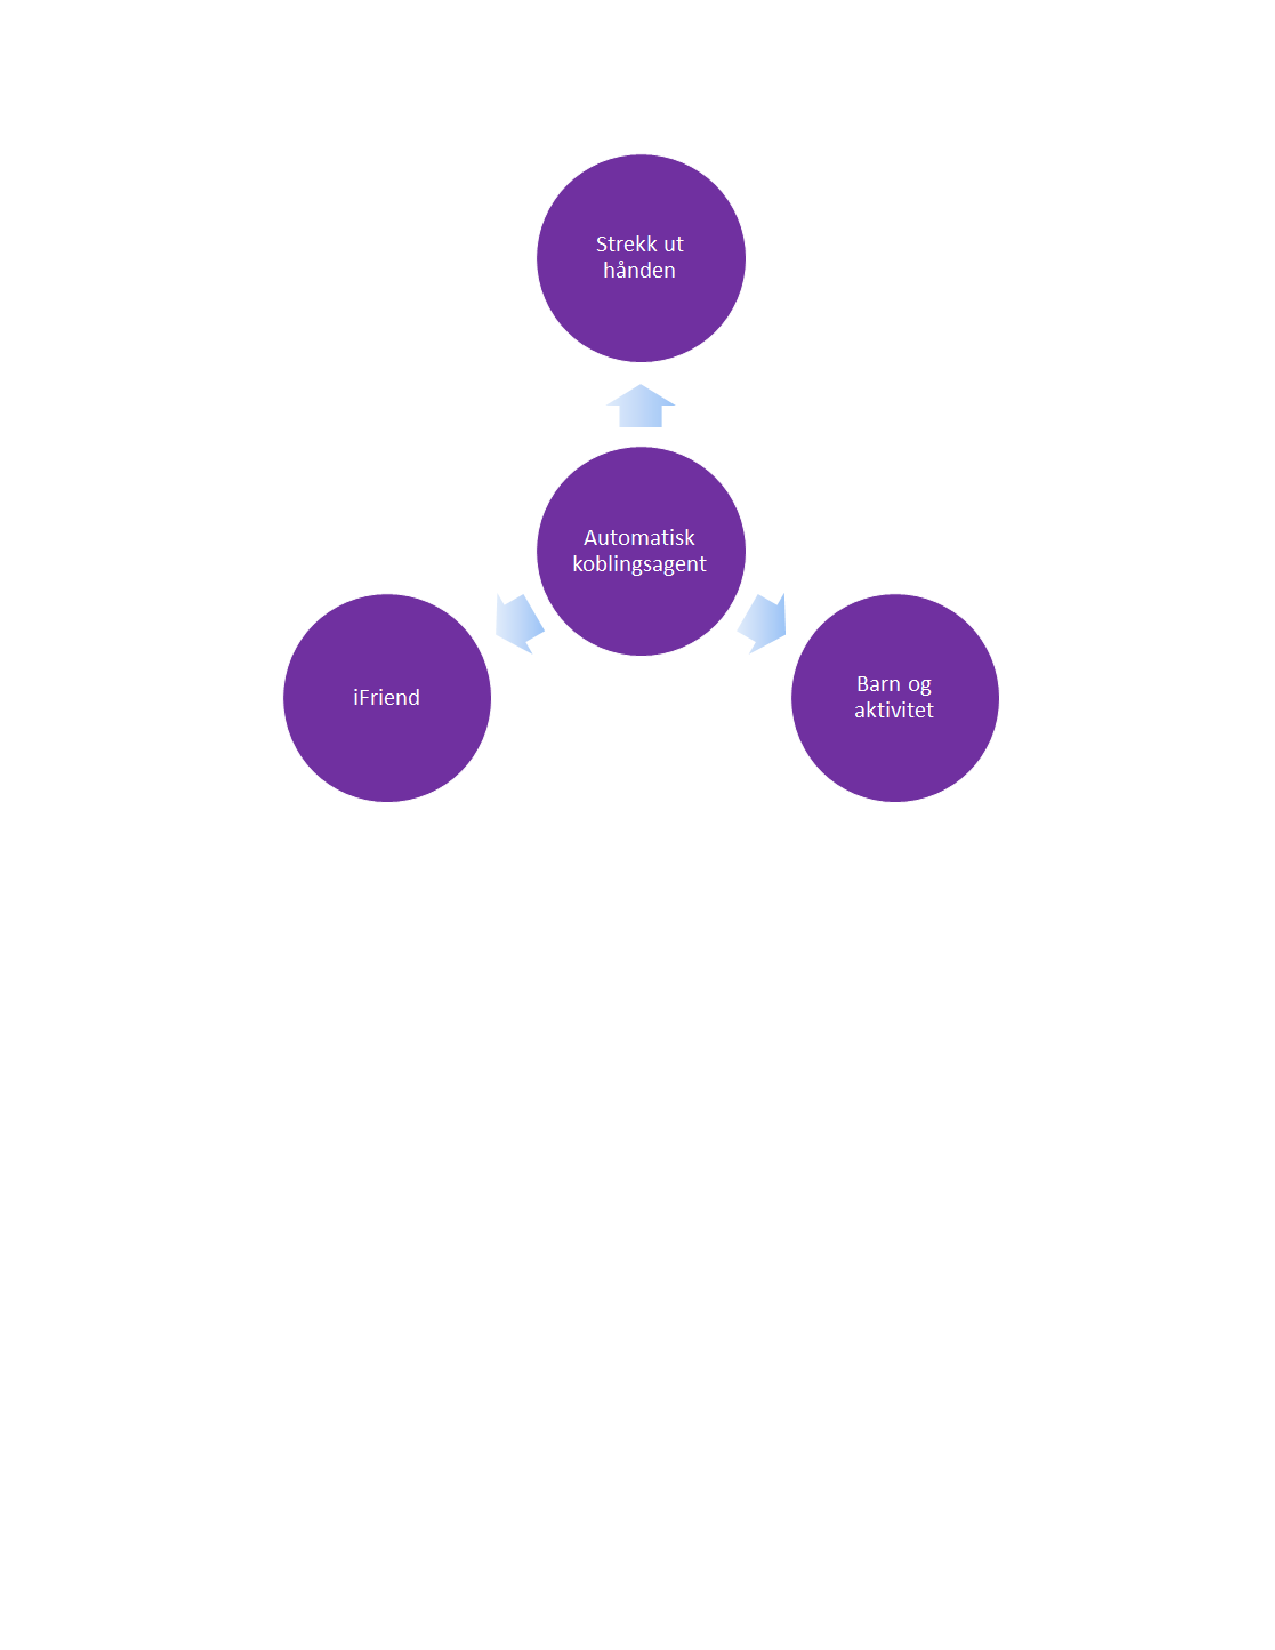
\includegraphics[clip=true, width=1 \textwidth,
trim=0cm 13cm 0cm 1cm]{automatiskKoblingsagent.pdf}
\captionof{figure}{Alternative bruksområder for en automatisk koblingsagent}
\label{fig:automatiskKoblingsagent}
\end{center}
